\documentclass{trlnotes}
\usepackage{trmath}
\addcompatiblelayout{commonplace}
\setlayout{commonplace}
\usepackage{trthm}
\usepackage{trsym} 
\usepackage{trphys}
% % \RequirePackage{stmaryrd}

% \RequirePackage{etoolbox}


%\RequirePackage{cmap}
% \RequirePackage{hyperref}
% \theoremstyle{definition}
% \newtheorem{thm}{Теорема}
% \newtheorem{de}{Определение}
% \newtheorem{lm}{Лемма}
% \newtheorem{exm}{Пример}
% \newtheorem{pr}{Свойство}
% \newtheorem{exc}{Упражнение}
% \newtheorem{cor}{Следствие}
% \newtheorem{st}{Утверждение}
% \theoremstyle{remark}
% \newtheorem{rem}{Замечание}
\newcommand*{\icom}{\ensuremath\text{\textit{,}}}
\newcommand*{\icol}{\ensuremath\text{\textit{:}}}
\newcommand*{\iscol}{\ensuremath\text{\textit{;}}}
\newcommand*{\com}{\ensuremath\text{\text{,}}}
\newcommand*{\col}{\ensuremath\text{\text{:}}}
\newcommand*{\scol}{\ensuremath\text{\text{;}}}
% \newcommand*{\so}{\ensuremath\Rightarrow}
\newcommand*{\bso}{\ensuremath\Leftarrow}
\newcommand*{\eqv}{\ensuremath\Leftrightarrow}
\newcommand*{\all}{\forall}
\newcommand*{\ex}{\exists \,}
% \newcommand*{\ov}{\overline}
\newcommand*{\un}{\underline}
\newcommand*{\ova}{\overrightarrow}
\newcommand*{\auth}[1]{\hfill \textit{#1}}
\newcommand*{\pd}{\partial}
% \newcommand*{\R}{\mathbb{R}}
% \newcommand*{\N}{\mathbb{N}}
\newcommand*{\DD}{\mathbb{D}}
\newcommand*{\K}{\mathbb{K}}
% \newcommand*{\C}{\mathbb{C}}
% \newcommand*{\C}{\mathbb{C}}
% \newcommand*{\Q}{\mathbb{Q}}
\newcommand{\An}{\wedge}
\newcommand{\Or}{\vee}
% \newcommand*{\Z}{\mathbb{Z}}
\newcommand*{\J}{\mathbb{J}}
\newcommand*{\bas}[2]{\overset{\vspace{-3pt}\tiny{\mb{#1}}}{#2}}
\newcommand*{\mc}{\mathcal}
\newcommand*{\mb}{\mathbf}
\newcommand*{\mf}{\mathfrak}
\newcommand*{\ti}{\textit}
\newcommand*{\la}{\langle}
\newcommand*{\ra}{\rangle}
\newcommand*{\tb}{\textbf}
\newcommand*{\mr}{\mathrm}
\newcommand*{\wt}{\widetilde}



% \DeclareMathOperator{\rk}{rk}
\DeclareMathOperator{\Dom}{Dom}
% \DeclareMathOperator{\id}{id}
\DeclareMathOperator{\Cl}{Cl}
% \DeclareMathOperator{\Res}{Res}
\DeclareMathOperator{\im}{Im}
% \DeclareMathOperator{\rot}{rot}
\DeclareMathOperator{\Div}{div}
% \DeclareMathOperator{\grad}{grad}
\DeclareMathOperator{\Id}{Id}
% \DeclareMathOperator{\Aut}{Aut}
% \DeclareMathOperator{\Stab}{Stab}
\DeclareMathOperator{\const}{const}

%\titleformat{\section}
%  {\sffamily\mdseries\upshape\LARGE}
%  {Билет \thesection:}{0.5em}{}



\usepackage{silence}
\WarningFilter{latex}{Reference}
\graphicspath{{../../img/}}
\newtagform{roman}[\renewcommand{\theequation}{\Roman{equation}}]()
\begin{document}
\paragraph{Краевая задача для ОДУ 2 порядка и сведение к задаче Коши}
\label{par:ode::bprobl}
\begin{defn}\label{defn:ode::bprobl}
  Рассмотрим ОДУ 2 порядка
  \[
    y'' + p(x) y' + q(x) y = f(x) \qquad y \in C^2([a;b])
  \]
  и 3 варианта условий на $y$
  \begin{enumerate}[I]
    \item $y(a) = A, \quad y(b) = B$ \label{it:ode::bprobl::cond:i}
    \item $y'(a) = A, \quad y'(b) = B$ \label{it:ode::bprobl::cond::ii}
    \item $y'(a) = α y(a) + A, \quad y'(b) = βy(b) + B$ \label{it:ode::bprobl::cond::iii}
    \end{enumerate}
  
  Если $y$~--- решение для которого выполнено какое-то из условий выше, то $y$~--- решение
  граничной задачи.
\end{defn}

\begin{defn}[Однородная краевая задача]\label{defn:ode::bprobl::hom}
  Положим $f \equiv 0$ в \ref{defn:ode::bprobl}.
\end{defn}
\begin{defn}[Однородные граничные условия]\label{defn:ode::bprobl::hombnd}
  Положим $A = B = 0$ в граничных условиях в \ref{defn:ode::bprobl}
\end{defn}

\begin{thrm}[об альтернативе]\label{thrm:ode::bprobl::alt}
  Рассмотрим однородную граничную задачу с однородными граничными условиями.
  Пусть $y_H$~--- решение однородной задачи. 

  Тогда
  \begin{enumerate}
    \item $y_0 \equiv 0$~--- единственное решение однородной задачи \so неоднородная краевая 
      задача имеет единственное решение
    \item $y_0 \equiv 0$~--- неединственное решение однородной задачи \so неоднородная краевая 
      задача имеет бесконечно много или не имеет решений вовсе
  \end{enumerate}
\end{thrm}


\begin{prf}
  Рассмотреть решение неоднородной краевой в виде $y(x) = y_0(x) + c_1 y_1(x) + c_2 y_2(x)$
  и подставить граничные условия, а дальше все следует из линейной алгебры.
\end{prf}


Разберёмся как численно найти $y_0, y_1, y_2$, потребовавшиеся в предыдущем доказательстве.
Будем считать что $p,q,f$ определены на $I \ni [a;b]$, так что $y$ можно продолжить 
на $(a-ε;b+ε)$. 
\begin{enumerate}
  \item $y(a) = 0$, $y'(a) = 0$. Поскольку $0$ явно решение однородной задачи, то что мы
    найдем будет как раз частным решением неоднородной задачи (Коши!).
  \item $y_H(a) = 1$, $y'_H(a) = 0$ и решаем мы тут однородную задачу (Коши!). Будем считать то что
    нашлось $y_1$
  \item $y_H(a) = 0$, $y'_H(a) = 1$. Скажем что это $y_2$. Здесь важно заметить про линейную
    независимость $y_1$ и $y_2$. Найдем определитель Вронского в точке $a$
    \[
      W = \begin{vmatrix}
        y_1(a) & y_2(a) \\
        y_1'(a) & y_2'(a) 
      \end{vmatrix} = 
      \begin{vmatrix}
        1 & 0 \\ 
        0 & 1 \\
      \end{vmatrix} = 1 \neq 0
    \]
    А тогда он нигде не ноль. А значит $y_1$ и $y_2$ линейно независимы.
\end{enumerate}

Всё это называется \emph{методом начальных данных} для решения краевой задачи.

В рассуждении выше можно было бы взять другие начальные данные дабы
упростить себе жизнь. Ведь никто не запрещает запихать, например, кусок $y_2$ в $y_0$
(если мы уже знаем правильное $c_2$). Нам просто были нужны какие-то линейно независимые
решения однородной задачи.

Рассмотрим граничную задачу в форме \ref{it:ode::bprobl::cond::iii}
\begin{enumerate}
  \item $y(a) = 0$, $y'(a) = A$, нашли  $y_0$.
  \item $y_H(a) = 1$, $y'_H(a) = α$, нашли $y_1$.
  \item $y_H(a) = 0$, $y'_H(a) = 0$. Мы просто решили что $y_2 \equiv 0$. Эту ЗК мы даже
    не решаем, а сразу знаем ответ.
\end{enumerate}
При таком раскладе $y(x) = y_0(x) + c_1 y_1(x)$. 
Проверим левое граничное условие 
\[
  \begin{split}
    y(a) &= y_0(a) + c_1\, y_1(a) = 0 + c_1 \, 1 = c_1 \\
    y'(a) &= y_0'(a) + c_1\, y_1'(a) = A + c_1 \, α = A + α\ y(a)
  \end{split}
\]
Как видно, всё получилось.

В случае \ref{it:ode::bprobl::cond:i} можно сделать так:
\begin{enumerate}
  \item $y(a) = A$, $y'(a) = 0$, нашли $y_0$.
  \item $y_H(a) = 0$, $y_H'(a) = 1$, нашли $y_1$.
\end{enumerate}
Как видно, свободы в выборе $c_1$ хватает чтобы разобраться с правой границей.

\begin{exmp}
  $y'' - q^2 y =0$, $y(0) = 1$, $y(b) = 1$

  \underdev, а он важный вообще-то, из него необходимость метода прогонки следует.
\end{exmp}

\paragraph{Метод дифференциальной прогонки}
\label{par:ode::difftdma}

Здесь будем решать краевую задачу с граничными условиями в форме \ref{it:ode::bprobl::cond::iii}.

Рассмотрим $α(x)$, $β(x) \that$ (прогоночные коэффициенты)
\begin{equation} \label{eq:ode::difftdma::tmda}
  y'(x) = α(x) \, y(x) + β(x)
\end{equation}
Такая форма напрашивается при вспоминании трюка, который мы делали в прошлом параграфе.
Там как раз $y'(a) = y_0(a) + c_1\, y_1(a)$, а $c_1 = y(a)$.
Здесь мы пока вводим прогоночные коэффициенты формально, а существование покажем конструктивно.

Найдем уравнения на $α, β$
\[
  \begin{aligned}
    y'  &= α y + β \\
    y'' &= α y' + α'y + β'
  \end{aligned} \so
  \begin{aligned}[t]
    &y'' + py' + qy = f \\
    \iff &αy' + α'y + β' + p (αy + β) + qy = f \\
    \iff &y\,(\underbrace{α^2 + α' + p α + q}_{0}) + \underbrace{α β + β' + pβ}_f = f 
  \end{aligned}
\]
В итоге получаем систему ОДУ первого порядка
\begin{equation}\label{eq:ode::difftdma::direct}
  \begin{aligned}
    α' &= - α^2 - p α - q \\
    β' &= f - pβ - αβ \\
  \end{aligned}
\end{equation}

Посмотрим что происходит на правом конце\footnote{а что делать если $α(b)=β$ неясно}
\[
  \begin{aligned}
    y'(b) &= α(b) y(b) + β(b) \\
    y'(b) &= β y(b) + B \\
  \end{aligned} \so y(b) = \frac{B- β(b)}{α(b) - β} 
\]
Сам метод выглядит так:
\begin{description}
  \item[прямая прогонка:] решаем систему \eqref{eq:ode::difftdma::direct} с начальными данными
    $α(a) = α$, $β(a) = A$.
  \item[обратная прогонка:] уже зная $α(x)$, $β(x)$ решаем \eqref{eq:ode::difftdma::tmda} c
    начальными данными $y(b) = \frac{B- β(b)}{α(b) - β}$.
\end{description}

\begin{rem}
  Рассмотрим однородную задачу с однородными граничными условиями. 
  Тогда \eqref{eq:ode::difftdma::tmda} переходит в $y'(x) = α(x) \, y(x)$.
  Если при этом $\exists\, c\in (a;b) \that y(c) = 0 \land y'(c) \neq 0$, то $α(c)$ не
  существует. Так что, как видно, не всякое решение краевой задачи можно найти методом
  прогонки.
\end{rem}

\paragraph{Метод прогонки для систем ОДУ}
\label{par:ode::tdmasys}

\begin{defn}\label{defn:ode::tdmasys::bprobl}
  Рассмотрим ОДУ
  \begin{equation}\label{eq:ode::tdmasys::ode}
    \v y' = \hat A(x) \,\v y + \v f(x) \qquad \v y \in C^2([a;b]), \quad y \colon [a;b]\to \R^s
  \end{equation}
  и условия вида
  \begin{equation*}\label{eq:ode::tdmasys::bndcond}
    \begin{aligned}
      x &= a& \hat α \v y(a) &= \v β &\qquad \hat α \colon \R^s \to \R^p \\
      x &= b& \hat γ \v y(b) &= \v δ &\qquad \hat γ \colon \R^s \to \R^q \\
        &   &                &       & s &= p+q
    \end{aligned}
  \end{equation*}
  
  Если $y$~--- решение для которого выполнено условие выше, то $y$~--- решение
  граничной задачи.
\end{defn}

\begin{rem}
  Вообще, граничные условия бывают куда более общего вида, но мы их не рассматриваем.
  То, что у нас~--- это линейные распадающиеся граничные условия.

  А вот так выглядят нераспадающиеся: 
  \[
    \hat α\v y(a) + \hat γ \v y(b) = \v β, \qquad \hat α,\hat γ\colon \R^s\to\R^s
  \]
\end{rem}

Общее решение задачи Коши~\ref{eq:ode::tdmasys::ode} имеет вид
\[
  \v y(x) = \v y_0(x) + \sum_{j=1}^s c_j \v y_j(x)
\]
где как обычно $y_0$~--- решение неоднородной задачи Коши, а $\{y_{j}\}$~--- фундаментальная
система решений однородной.

\clause{Метод начальных данных} такой же в \ref{par:ode::bprobl}~--- находим
из граничных условий $\{c_j\}$ в общем решении.

Чтобы добыть решения задач Коши можно взять $\v y_j(a) = \v e_j$
(это единичный вектор с 1 на $j$ом месте), $\v y_0 (a) =0$

Можно снова уменьшить количество работы
% в этом месте было потеряно больше часа на поиск н.д в явном виде
\begin{enumerate}
  \item в качестве начальных данных для $y_0$~--- какое-нибудь решение системы $\hat α y = β$
  \item в качестве начальных данных для $y_j$, $j\in {p+1}\intrng {s}$~--- $q$ линейно независимых
    решений $\hat αy = 0$
  \item $y_j \equiv 0$, $j \in 1\intrng p$
\end{enumerate}

В итоге решение примет вид 
\[
  \v y(x) = \v y_0 (x) + \sum_{j=p+1}^{s} c_j \v y_j(x) 
\]

\plholdev{здесь снова этот понятный кусок про экспоненты и беды вычислений}\underdev

\clause{Метод прогонки,} в котором cнова зададим $\hat α, \v β$
\begin{equation}\label{eq:ode::tdmasys::tdma}
  \hat α(x) \, \v y(x) = \v β(x),  \qquad \hat α \colon [a;b]×\R^s \to \R^p 
\end{equation}
При таком условии $\forall\, x\holds y(x)\in M \subset \R^s$, $\dim M = s-p$ 
(предполагая что $\rk \hat α(x) = p$) 

Найдем уравнения на $\hat α(x), \v β(x)$
\[\bindvectors{y,β,f}\bindqoperators{α, A}% weeell, they just look simular
  \begin{aligned}
    α y &= β \\
    α y' +  α' y&=  β' \\
  \end{aligned} \so
  \begin{aligned}[t]
    &y' = Ay + f  \\
    &αAy  + αf + α'y  = β' \\
    \iff &(\underbrace{αA + α'})\,y - \underbrace{β'} = - αf 
  \end{aligned}
\]

Пусть $α_j$~--- строка $\hat α$.
Тогда мы получаем систему ОДУ первого порядка
\begin{equation}\label{eq:ode::tdmasys::direct}
  \begin{aligned}
    α_j' &= - \hat A^T \, α_j \\
    β_j' &= (α_j,\v f) \\
  \end{aligned}
\end{equation}

Посмотрим что происходит на правом конце
\begin{equation}\label{eq:ode::tdmasys::rightbndcond}
  \left\{\begin{aligned}
    \hat α(b) \, \v y(b) &= \v β(b) \\
    \hat γ \v y(b) &= \v δ \\
  \end{aligned}\right. 
\end{equation}
это просто линейная система порядка $s$ на $\v y(b)$, решаем и находим.

Сам метод выглядит так:
\begin{description}
  \item[прямая прогонка:] решаем прогоночные уравения\eqref{eq:ode::tdmasys::direct}
    с начальными данными $\hat α(a) = \hat α$, $\v β(a) = \v β$.
  \item[обратная прогонка:] уже зная $α(x)$, $β(x)$ решаем \eqref{eq:ode::tdmasys::tdma} c
    начальными данными $y(b)$, найденным из системы \eqref{eq:ode::tdmasys::rightbndcond}.
\end{description}

\begin{rem}\quest{}
  Метод с заменой $\hat A$ на сопряженную в прогоночных уравениях 
  уже пафосно называется методом \emph{сопряжённых систем}, но ничем кроме
  названия по сути не отличается.
\end{rem}

\begin{rem}
  Вообще, этот метод накладывает слишком жёсткие условия на $\hat α$, $\b β$.
  Например краевая задача из~\ref{par:ode::bprobl} им не решается. 
  Проблема возникает в том месте, где из $(\hat α\hat A + \hat α')\,\v y = 0$ выводится
  $\hat α\hat A + \hat α' =0$. Произвольностью $\v y$ мы вообще-то пользоваться не можем,
  так как на него есть условие $\hat α(x) \, \v y(x) = \v β(x)$.
\end{rem}

\begin{rem}
  У вышеописанного метода есть ещё пара недостатков:
  \begin{enumerate}
    \item $α_j' = -\hat A^T\, α_j$ отличается от исходной системы только отсутствием
      неоднородности, так от проблем связанных с потерей точности из-за собственных
      чисел разного знака в решениях задач Коши мы убежать не смогли.
    \item $\hat α \hat α^T$ может быть плохо обусловленной и ища $\v y(b)$ мы потеряем точность.
      \note{
      $\rk \hat α \hat α^T \geqslant 2\rk \hat α - s$ из теоремы Сильвестра о ранге,
    так что так в одну сторону вроде можно}
  \end{enumerate}

  Собственно, для того чтобы обойти эти проблемы и нужен \ref{par:ode::orthtdma}.
\end{rem}

\paragraph{Ортогональная прогонка}
\label{par:ode::orthtdma}

<<будем решать немного другую задачу>>

Заменим уравенение для $\hat α$ в методе выше.

\[\bindqoperators{α, A}
  α' = - αA \longrightarrow  α' = - α A + αA α^T \left(α α^T\right)^{-1} α
\]

Крокодил в формуле сверху~"--- ортогонанальная проекция $\hat α \hat A$ на $\hat α$,
а скалярное произведение имеет вид $(\hat α, \hat β) = \hat α \hat β^T$\note{
  на самом деле оно несимметрично. Нужно здесь понимать матрицу как набор векторов-строк.
  Тогда какой-то смысл есть.
}.
Так что по идее, раз мы проекцию на $\hat α$ вычли, $(\hat α',\hat α) = 0$.
Проверим:
\[\bindqoperators{α, A}
  α' α^T = -α A α^T + αA α^T \left(α α^T\right)^{-1} αα^T  = -α A α^T + αA α^T = 0
\]
Отсюда следует, что $\fder{}{x} \left( \hat α \hat α^T \right) = 0$, так что
матрица $\hat α \hat α^T$ постоянна на всём $[a;b]$

Получим уравнения на прогоночные коэффициенты
\[\bindvectors{y,β,f}\bindqoperators{α, A}% weeell, they just look simular
  \begin{aligned}[t]
    &αAy  + αf + α'y  = β' \\
    \iff &αAy + αf  -αAy + αAα^T \left(α α^T\right)^{-1} \underbrace{αy}_{β} = β'
  \end{aligned} 
\]
В итоге
\begin{equation}\label{eq:ode::orthtdma::tdma}
  \bindvectors{y,β,f}\bindqoperators{α, A}
  \begin{aligned}
    α' &=  - α A + αA α^T \left(α α^T\right)^{-1} α \\
    β' &= αf + αAα^T \left(α α^T\right)^{-1} β
  \end{aligned} 
\end{equation}

Разберёмся что делать с $\left(α α^T\right)^{-1}$. Не очень приятно каждый раз искать обратную 
матрицу.

На левой границе $\hat α(a) \v y(a) = \v β(a)$. Проведём процесс Грамма-Шмидта и 
ортогонализуем строчки $\hat α(a)$.
При этом заменили переменную в исходном уравении, соответственно поменялись 
$\hat A\to \hat B$, $\v f\to \v g$. Зато $\hat α(a)\, \hat α(a)^T = I$.
Так что прогоночные уравения принимают вид
\begin{equation}\label{eq:ode::orthtdma::orthtdma}
  \bindvectors{y,β,g}\bindqoperators{α, B}
  \begin{aligned}
    α' &=  - α B + αB α^T α \\
    β' &= αg + αBα^T β
  \end{aligned} 
\end{equation}

Поскольку $\hat α\hat α^T$ постоянна на $[a;b]$ (всюду $I$),
то проблем с её плохой обусловленностью в $x=b$ нет. Правое граничное условие
решится.

Судя по всему, это же условие исключает быстрый рост компонент $\hat α$.
Так что обе проблемы из замечания в конце предыдущего параграфа снимаются.
\quest\note{про это два слова в Крылове написано и больше нигде нет.}

Вышеописанный метод ещё называется методом Абрамова.


\paragraph{Разностный метод для краевой задачи 2 порядка}
\label{par:ode::findiff}
\begin{aux}
  \textit{Предупреждение:}
  в силу повышенной техничности этого параграфа он написан в соответствующем стиле.
  Что поделать. Приятного прочтения.
\end{aux}

Решать краевую задачу для дифференциального уравения второго порядка
\begin{equation}
  y'' + p(x) y' + q(x) y = f(x) \qquad y \in C^2([a;b]) \label{eq:ode::findiff::ode}
\end{equation}

\clause{Алгоритм}
\begin{defn}[Метод разностной прогонки]\label{defn:ode::findiff::alg}
  Пусть задано дифференциальное уравнение с граничными условиями.
  Методом разностной прогонки называет следующий алгоритм:
  \begin{enumerate}
    \item Выбор сетки: узлы, шаг (если она равномерная)
    \item Построение сеточных уравений
      \begin{enumerate}
        \item Диффур в узлах сетки
        \item Все производные через конечные разности
      \end{enumerate}
    \item Решение получившейся линейной системы
  \end{enumerate}
\end{defn}

Будем дальше всюду считать, что решение задано на $[a;b]$
\[
  \text{$n$ узлов}\qquad h = \frac{b-a}{n} \qquad x_k = a + kh
\]
\clause{Формулы численного дифференцирования} 
Здесь $M_n = \max \abs{y^{(m)}(x)}$
\begin{align}
  \label{eq:ode::findiff::simpforward}
  y'(x) &= \frac{y(x+h) -y (x)}{h} + R & \abs{R} &\leqslant \tfrac{hM_2}{2} \\
  \label{eq:ode::findiff::simpbackward}
  y'(x) &= \frac{y(x) - y (x-h)}{h} + R & \abs{R} &\leqslant \tfrac{hM_2}{2} \\
  \label{eq:ode::findiff::threepointforward}
  y'(x) &= \frac{-y(x+2h) + 4y (x+h) - 3y(x)}{2h} + R & \abs{R} &\leqslant \tfrac{h^2M_3}{3} \\
  \label{eq:ode::findiff::threepointbackward}
  y'(x) &= \frac{3y(x) - 4y (x-h) + y(x-2h)}{2h} + R & \abs{R} &\leqslant \tfrac{h^2M_3}{3} \\
  \label{eq:ode::findiff::simmetric}
  y'(x) &= \frac{y(x+h) - y (x-h)}{2h} + R & \abs{R} &\leqslant \tfrac{h^2M_3}{6} \\
  \label{eq:ode::findiff::simmetricsecondorder}
  y''(x) &= \frac{y(x+h) - 2y (x) + y(x-h)}{h^2} + R & \abs{R} &\leqslant \tfrac{h^2M_4}{12}
\end{align}
Cхемы \ref{eq:ode::findiff::simpforward} и \ref{eq:ode::findiff::simpbackward} называются 
простейшими.

\clause{Разностное уравнение}

\begin{equation*}
  \frac{y(x_{k+1}) - 2y(x_k) + y(x_{k-1})}{h^2} + R_1 
  + p(x_k) \, \frac{y(x_{k+1}) - y(x_{k-1})}{2h} + p(x_k)\,R_2 
  + q(x_k) \, y(x_k) = f(x_k)
\end{equation*}

Можно заметить, что $R_1 + p(x_k)\, R_2 = O(h^2)$.
Так что можно вместо $y(x_k)$ получить приближённое решение $y_k$
(по сути, решение уже совсем другой задачи). Попутно, обозначим
\[
  p(x_k) = p_k,\qquad q(x_k) = q_k, \qquad f(x_k) = f_k.
\]
Получится
\begin{equation}\label{eq:ode::findiff::diffeq}
  \frac{y_{k+1} - 2y_k + y_{k-1}}{h^2}
  + p_k \, \frac{y_{k+1} - y_{k-1}}{2h} 
  + q_k \, y_k = f_k
\end{equation}

\clause{Граничные условия} будут рассматриваться \ref{it:ode::bprobl::cond::iii} типа,
но вообще это неважно. Всё равно раскрывать не будем.

\begin{enumerate}
  \item \emph{Трёхточечная односторонняя аппроксимация}
      \begin{equation*}
        y'(x) = \frac{-y(x+2h) + 4y(x+h) - 3 y(x)}{2h} + O(h^2)
      \end{equation*}

      Запишем это выражение для границ:
      \begin{alignat*}{3}
        y'(a) &= \frac{-y(a+2h) + 4y(a+h) - 3 y(a)}{2h} + O(h^2) 
              &\quad&\to\quad &
        αy_0 + A &= \frac{-y_2 + 4 y_1 - 3y_0}{2h}\\
        y'(b) &= \frac{3y(b) - 4y(b-h) + y(b-2h)}{2h} + O(h^2) 
              &\quad&\to\quad &
        βy_n + B &= \frac{3y_n - 4 y_{n-1} + y_{n-2}}{2h}
      \end{alignat*}
    \item \emph{Метод фиктивных узлов}
      \begin{enumerate}
        \item Введём $y_{-1} = y(a-h)$, $y_{n+1} = y(b+h)$
          \begin{equation*}
            y'(x) = \frac{y(x+h) - y(x-h)}{2h} + O(h^2)
          \end{equation*}

          Запишем это выражение для границ:
          \begin{alignat*}{3}
            y'(a) &= \frac{y(a+h) - y(a-h)}{2h} + O(h^2) 
                  &\quad&\to\quad &
            αy_0 + A &= \frac{y_1 - y_{-1}}{2h}\\
            y'(b) &= \frac{y(b+h) - y(b-h)}{2h} + O(h^2) 
                  &\quad&\to\quad &
            βy_n + B &= \frac{y_{n+1} - y_{n-1}}{2h}
          \end{alignat*}
          Как правило, решение можно продолжить с отрезка на интервал побольше, подберём
          $h \that y(a-h) \in I \land y(b+h) \in I$. Так что такой метод имеет смысл.
        \item Сдвинем сетку на $\lfrac h2$, $x_0 = a-\lfrac h2$, $x_{n+1} = b+\lfrac h2$
          \[
            x_k = a- \lfrac h2 + kh \qquad k = 0,1 \intrng n+1
          \]
          Значения в узлах сетки при этом придётся вводить с помощью интерполяции
          \[
            y(a) = \frac{y(a-\lfrac{h}2) + y(a+\lfrac{h}2)}{2}
          \]
          Сами выражения для производной имеют вид
          \begin{equation*}
            y'(x) = \frac{y(x+\lfrac h2) - y(x-\lfrac h2)}{h} + O(h^2)
          \end{equation*}

          Запишем это выражение для границ:
          \begin{alignat*}{3}
            y'(a) &= \frac{y(a+\lfrac{h}2) - y(a-\frac{h}2)}{h} + O(h^2) 
                  &\quad&\to\quad &
            α\, \frac{y_0 + y_1}{2} + A &= \frac{y_1 - y_{0}}{h}\\
            y'(b) &= \frac{y(b+\lfrac h2) - y(b-\lfrac h2)}{h} + O(h^2) 
                  &\quad&\to\quad &
            β\, \frac{y_{n+1} + y_n}{2} + B &= \frac{y_{n+1} - y_{n}}{h}
          \end{alignat*}

          Такой подход не очень удобен если нужны значения в узлах. Придётся уменьшать шаг
          в $2$ раза.
      \end{enumerate}
    \item \emph{Использование ДУ для исключения главного члена простейшей формулы}\par
        \begin{equation*}
          y'(x) = \frac{y(x+h) - y(x)}{h} + R, \quad R = O(h)
        \end{equation*}
        Теперь запишем разложение в ряд Тейлора:
        \begin{equation*}
          y(x+h) = y(x) + h y'(x) + \frac{h^2}{2}y''(x) + O(h^3) 
          \iff y'(x)  = \frac{y(x+h) - y(a)}{h}  - \frac h2 y''(x) + O(h^2)
        \end{equation*}
        Из исходного уравнения \eqref{eq:ode::tdmasys::ode} подстановкой простейшей формулы получаем
        \begin{align*}
          y''(x) &= -\bigl(p(x) y'(x) + q(x) y(x) \bigr) + f(x)  
          = -\left(p(x) \,\tfrac{y(x+h) -y(x)}{h} + p(x) O(h) + q(x) y(x) \right) + f(x)
          \notag \\
          \so 
          -\tfrac{h}{2} y''(x) &= \tfrac{p(x)}{2} \Bigl(y(x+h) - y(x)\Bigr) + 
          \tfrac{h}{2} \Bigl(q(x)y(x) - f(x)\Bigr) + O(h^2)
        \end{align*}
        
        Оценка производной на краю
        \begin{align*}
          y'(a) &= \frac{y(a+h) - y(a)}{h} + \frac{p(a)}{2} \biggl(y(a+h) - y(a)\biggr) + 
          \frac{h}{2} \biggl(q(a) y(a) - f(a)\biggr) + O(h^2)\\
          y'(b) &= \frac{y(b) - y(b-h)}{h} - \frac{p(b)}{2} \biggl(y(b) - y(b-h)\biggr) - 
          \frac{h}{2}\,\biggl(q(b) y(b) - f(b)\biggr) + O(h^2)
        \end{align*}

        На сетке оно имеет вид
        \begin{equation*}
          \begin{split}
            α y_0 + A &= \frac{y_1 - y_{0}}{h} + \frac{p_0}{2} \biggl(y_1 - y_{0}\biggr)
            + \frac{h}{2}\,\biggl(q_0 y_0 - f_0\biggr) \\
            β y_n + B &= \frac{y_n - y_{n-1}}{h} - \frac{p_n}{2} \biggl(y_n - y_{n-1}\biggr)
            - \frac{h}{2}\,\biggl(q_n y_n - f_n\biggr) \\
            \end{split}
        \end{equation*}
\end{enumerate}

\clause{Составление системы линейных уравнений}
\begin{equation}\label{eq:ode::findiff::tdma}
  \begin{aligned}
    c_0 y_1     &- b_0 y_0                  &&=& &d_0 \\
    c_k y_{k+1} &- b_k y_k+ y_{k-1} a_k     &&=& &d_k,\quad k= 1\intrng n-1 \\
                &- b_n y_n + a_n y_{n-1}    &&=& &d_n 
  \end{aligned}
\end{equation}
Из разностного уравнения \eqref{eq:ode::findiff::diffeq} можно найти $a_k, c_k, b_k, d_k$
\[
  \begin{aligned}
    a_k &= 1- \tfrac{h}2 \, p_k &
    b_k &= 2- h^2 \, q_k &
    c_k &= 1+ \tfrac{h}2 \, p_k &
    d_k &= {h}^2 \, f_k 
  \end{aligned}
\]

Явные выражения для $a_0, b_0, c_0, d_0$ и $a_n, b_n, c_n, d_n$
зависят от способа учета граничных условий. Разве что $a_0 = 0\land c_0 = 0$.
Оставим остальные читателям из Беларуси в качестве упражнения.

\paragraph{Метод разностной прогонки}
\label{par:ode::fintdma}
Вспомним систему линейную систему~\ref{eq:ode::findiff::tdma}.
Её матрица, как видно чуть ниже, трёхдиагональная.
\[
  \begin{pmatrix}
    -b_0   & c_0    &         &          & 0       \\
    a_1    & -b_1   & c_1     &          &         \\
           & \ddots & \ddots  & \ddots             \\
           &        & a_{n-1} & -b_{n-1} & c_{n-1} \\
    0      &        &         & a_n      & -b_n    \\
  \end{pmatrix}
\]
Такие СЛУ можно решать не за $O(n^3)$, а за $O(n)$. Опишем, как именно.


Преобразум систему: уберём поддиагональ, на самой диагонали оставим всюду 1.
Тогда можно написать прогоночное соотношение, очень похожее на такое же для 
дифференциальной прогонки (в \ref{par:ode::difftdma}). 
\begin{equation}\label{eq:ode::fintdma::direct}
  y_k = α_k y_{k+1} + β_k
\end{equation}

% спёр из своего отчёта: там слишком хорошо, мне лучше не сделать
Свяжем $α, β$ с $a, b, c, d$.
\[
  \left\{
  \begin{aligned}
    &y_{k-1} = α_{k-1} y_k + β_{k-1} \\
    &a_k y_{k-1} - b_k y_k + c_k y_{k+1} = d_k
  \end{aligned}\right. 
  \so
  \begin{aligned}[t]
         &a_k α_{k-1} y_{k} + a_k β_{k-1} - b_k y_k + c_k y_{k+1} = d_k \\
    \iff &y_k = \frac{c_k}{b_k - a_k α_{k-1}}y_{k+1} + \frac{a_k β_{k-1} - d_k}{b_k - a_k α_{k-1}}
  \end{aligned}
\]

Отсюда получаются удобные рекурсивные соотношения для $α_k, β_k$
\begin{equation}\label{eq:ode::fintdma::tdmaeq}
  α_k = \frac{c_k}{b_k - a_k α_{k-1}}; \qquad β_k = \frac{a_k β_{k-1} - d_k}{b_k - a_k α_{k-1}}
\end{equation}
Начальные значения $α_k, β_k$ легко определяются из линейной системы на
$a_k, b_k, c_k, d_k$ \eqref{eq:ode::findiff::tdma}.

Итак, алгоритм, следующий
\begin{description}
  \item[прямая прогонка:] решаем прогоночные уравения~\eqref{eq:ode::fintdma::tdmaeq}
    с начальными данными $α_0 = \frac{c_0}{b_0}$, $β_0 = -\frac{d_0}{b_0}$.
  \item[обратная прогонка:] уже зная $α_k$, $β_k$ решаем прогоночное соотношение 
    \eqref{eq:ode::fintdma::direct} c
    начальными данными $y_n = β_n$ ($c_n = 0 \so α_n = 0$).
\end{description}

Как видно, что прямая, что обратная прогонка имеют асимптотику $O(n)$, что не может не
радовать.
Теперь подумаем над корректностью метода.
\paragraph{Лемма об оценке для системы разностных уравений}
\label{par:ode::diffeqest}

\begin{prop}[Достаточное условие]\label{prop:ode::diffeqest::suff}
  Пусть $\forall k\holds a_k, c_k > 0$ ($c_n, a_0 = 0$), и СЛУ имеет
  диагональное преобладание: $b_k \geqslant a_k + c_k$.

  Тогда если $\exists\, k\that b_k > a_k + c_k$ 
  прогоночные уравнения \ref{eq:ode::fintdma::tdmaeq} разрешимы
\end{prop}
\begin{prf}
  Проблемы у нас возникнут только если знаменатели обратятся в $0$.
  Учитывая диагональное преобладание, это эквивалентно $α_{k-1} \geqslant 1$.
  
  \gprov $0 < α_{k-1} \leqslant 1$ (по индукции)
  \begin{description}
    \item[база:] $α_0 = \frac{c_0}{b_0}$, $b_0 \geqslant c_0 > 0$, $c_0 \leqslant b_0$.
      Кажется, все верно.\note{здесь бы и хотелось сразу $α_0 < 1$, да $a_0 = 0$, 
      так что неравенство $c_0 \leqslant b_0$ нестрогое}
    \item[переход:] Знаем что $α_{k-1} \leqslant 1$. 
      Так что из условий теоремы
      \[
        b_k - α_{k-1} a_k \geqslant b_k - a_k \geqslant c_k > 0 \so 
        0< α_k = \frac{c_k}{b_k - a_k α_{k-1}} \leqslant 1
      \]
      Если $α_{k-1} < 1$, то $α_k < 1$, поскольку $b_k - α_{k-1} a_k > b_k - a_k$.
      Это означает, что если уж неравенство стало строгим, оно таким и останется.
  \end{description}
  Таким образом, все знаменатели кроме последнего $>0$.  В нём $c_n = 0 \ngtr 0$.
 
  Разберёмся, что с ним делать.
  Поскольку мы предположили что диагональное преобладание хоть где-то строгое 
  (в $k_0$), возможны варианты:
  \begin{enumerate}
    \item $k_0 < n \so α_{n-1} < 1$. Тогда $b_n -a_n α_{n-1} > b_n - a_n \geqslant 0$ 
    \item $k_0 = n \so α_{n-1} \leqslant 1$. Тогда $b_n -a_n α_{n-1} \geqslant b_n - a_n > 0$ 
  \end{enumerate}
  Как видно, даже последний знаменатель $\neq 0$
\end{prf}

Посмотрим, какие условия утверждение выше накладывает на уравнение.
Вспомним выражения для $a_k, \ldots$
\[
  \begin{aligned}
    a_k &= 1- \tfrac{h}2 \, p_k &
    b_k &= 2- h^2 \, q_k &
    c_k &= 1+ \tfrac{h}2 \, p_k &
    d_k &= {h}^2 \, f_k 
  \end{aligned}
\]
Отсюда
\[
  \begin{aligned}
    a_k &> 0 &&\Leftarrow& h &< \tfrac{2}{\max \abs{p_k}}\\
    c_k &> 0 &&\Leftarrow& h &< \tfrac{2}{\max \abs{p_k}} \\
    b_k &\geqslant c_k + a_k &&\iff& &\framebox{$q_k \leqslant 0$}
  \end{aligned}
\]
Можно ещё подумать про граничные условия. Тут всё зависит от способа вычисления производной на
границе.
\begin{exmp}
  Оценим производную по простейшей схеме
  \[
    \frac{y_1-y_0}{h} = αy_0 + A
  \]
  Тогда 
  \[
    y_1 + y_0 (-1 - αh) = Ah \so \begin{aligned}
      b_0 &= 1+ αh \\
      c_0 &= 1
    \end{aligned}
  \]
  И по сути нам нужно \framebox{$α \geqslant 0$}.
  Аналогично с правой границей, там \framebox{$β \leqslant 0$}.
\end{exmp}

Если хотя бы одно из трёх условий в рамке строгое, прямая прогонка сработает.

\begin{rem}
  Рассмотрим однородную задачу с однородным левым граничным условияем (\hbox{$A=0$}).
  Тогда $d_k = 0 \so β_k = 0$ при $k<n$. Прогоночное соотношение примет вид $y_k = α_k y_{k+1}$.
  Если один из узлов находится вблизи $y(x) = 0$, $α_k$ окажется большим, что не очень
  хорошо с вычислительной точки зрения. Но, вообще, вероятность этого низкая, и можно просто узлы
  сдвинуть если что-то сломается.
\end{rem}

Теперь видимо то, что в названии
\begin{lem}\label{lem:ode::finddivconv::est}
  Пусть выполено условие достаточности прогонки \ref{prop:ode::diffeqest::suff} в усиленном 
  виде: \[
    b_k \geqslant a_k + c_k + δ,\quad δ > 0.
  \]
  Тогда
  \[
    \max_k \abs{y_k} \leqslant δ^{-1} \max_k \abs{d_k}
  \]
\end{lem}

\begin{prf}
  Пусть $M = \max \abs{y_k} = y_{k_0}$ (их же конечное число).
  Тогда из разностной СЛУ \eqref{eq:ode::findiff::tdma}
  \[
    \begin{split}
      b_{k_0} y_{k_0} &= a_{k_0} y_{k_0-1} + c_{k_0} y_{k_0+1} + d_{k_0}\\
      \so b_{k_0} M & \leqslant a_{k_0} M + c_{k_0} M + d_{k_0} \\
                    &\so δM \leqslant (b_{k_0} - a_{k_0} - c_{k_0}) \, M \leqslant \abs{d_{k_0}} 
      \leqslant \max \abs{d_k} 
    \end{split}
  \]
\end{prf}
\paragraph{Теорема о сходимости разностного метода}
\label{par:ode::finddivconv}


\begin{thrm}\label{thrm:ode::finddivconv::conv}
  Рассмотрим краевую задачу \ref{it:ode::bprobl::cond::iii} типа для уравнения второго порядка.
  Пусть 
  \begin{enumerate}
    \item $p, q, f \in C^2([a;b])$
    \item $q(x) \leqslant -q_0$, $q_0 > 0$
    \item $α < 0$, $β > 0$
  \end{enumerate}
  Тогда разностный метод сходится: 
  \[
    \forall \, k \holds \abs{y(x_k) - y_k} < Ch^2, \quad C=\mathrm{const}
  \]
\end{thrm}

\begin{prf}
  Запишем уравнение на сетке:
\begin{equation*}
  \frac{y(x_{k+1}) - 2y(x_k) + y(x_{k-1})}{h^2} + R_1 
  + p(x_k) \, \frac{y(x_{k+1}) - y(x_{k-1})}{2h} + p(x_k)\,R_2 
  + q(x_k) \, y(x_k) = f(x_k)
\end{equation*}
Вычтем теперь из него разностное (которое \eqref{eq:ode::findiff::diffeq}),
вводя $w_k = y(x_k) - y_k$
\[
  \frac{w_{k+1}- 2w_k + w_{k-1}}{h^2} + p_k\,\frac{w_{k+1} - w_{k-1}}{2h} + q_k\,w_k = R,
  \quad R = -R_1 - p_k R_2
\]
Если вспомнить как выглядят оценки $R_1$ и $R_2$ то становится понятно зачем нужен первый пункт
в условиях теоремы. Но мы вспоминать точный вид не будем, а просто запишем $R = Lh^2$

Чтобы оценить произодную на границе, можно воспользоваться формулой с фиктивными узлами 
и сдвинутой сеткой (на $\lfrac{h}2$), тогда:
\[
  \frac{w_1 - w_0}{h} = α \frac{w_0 + w_1}{2} + R_0\quad 
  \frac{w_{n+1} - w_n}{h} = β \frac{w_{n+1} + w_n}{2} + R_{n+1}
\]
Выражения для $R$ снова квадратичны по $h$, запишем их так: $R_0 = L_0 h^2$, $R_{n+1} =
L_{n+1}h^2$.

Запишем выражения для коэффициентов линейной системы c $w_k$:
\[
  \begin{aligned}
    a_k &= \tfrac{1}{h^2} - \tfrac{p_k}{2h} &
    b_k &= \tfrac{2}{h^2} - q_k &
    c_k &= \tfrac{1}{h^2} + \tfrac{p_k}{2h} &
    d_k &= {h}^2 L 
  \end{aligned}
\]
(они такие же как и раньше, только правая часть в уравении поменялась)

Подгоним под условия леммы~\ref{lem:ode::finddivconv::est}
\[
  b_k \geqslant a_k + c_k + δ \iff -q_k  \geqslant δ \;\Leftarrow\; δ = q_0
\]

На границах
\[
  \begin{aligned}
    a_0 &= 0 &
    b_0 &= \tfrac{1}{h} + \tfrac{α}2 &
    c_0 &= \tfrac{1}h - \tfrac{α}2 &
    d_0 &= {h}^2 L_0 \\
    a_{n+1} &= \tfrac{1}h + \tfrac{β}2  &
    b_{n+1} &= \tfrac{1}h - \tfrac{β}2 &
    c_{n+1} &= 0 &
    d_{n+1} &= -{h}^2 L_{n+1} \\
  \end{aligned}
\]

Снова найдём $δ$
\[
  \begin{aligned}
    b_0 &\geqslant a_0 + c_0 + δ &&\iff& α &\geqslant δ &&\Leftarrow& δ &= α \\
      b_{n+1} &\geqslant a_{n+1} + c_{n+1} + δ &&\iff& -β &\geqslant δ &&\Leftarrow& δ &= -β \\
  \end{aligned}
\]

Выберем:
\[
\begin{aligned}
  δ &= \min \left\{q_0, α, -β\right\} & C &= \max \left\{\abs{L}, \abs{L_0}, \abs{L_1}\right\}
\end{aligned}  
\]

Тогда по лемме 
\[
  \max \abs{w_k} \leqslant δ^{-1}\max \abs{d_k} \so \max\abs{y(x_k) - y_k} \leqslant δ^{-1} C h^2
\]
\end{prf}

\plholdev{дальше идет каша из всяких обобщений, не буду пока их писать}


\paragraph{Жёсткие системы ОДУ}
\label{par:ode::stiff}

Будем рассматривать задачу Коши для системы обыкновенных дифференциальных уравнений.
\[
  \v y'(x) = f(x, \v y(x)), \qquad \v y(x_0) = \v y_0
\]
Пусть $x_n$~--- узлы равномерной сетки с шагом $h$.

\clause{Методы численного интегрирования ОДУ} 
\begin{enumerate}
  \item Метод Эйлера\label{it:ode::stiff::methods::euler}
    \[\bindvectors{y}
      y_{n+1} = y_n + h f(x_n, y_n)
    \]
  \item Неявный метод Эйлера\label{it:ode::stiff::methods::impeuler}
    \[\bindvectors{y}
      y_{n+1} = y_n + h f(x_{n+1}, y_{n+1})
    \]
\end{enumerate}
оба метода выше имеют ошибку $\sim O(h)$. Поэтому они и называются простейшими.

Рассмотрим более точные методы
\begin{enumerate}[resume]
  \item Улучшенный метод Эйлера\label{it:ode::stiff::methods::enheuler}
    \[\bindvectors{y}
      y_{n+1} = y_n + \frac{h}{2} \biggl( f(x_n,y_n) + f\bigl(x_{n+1}, y_n + hf(x_n, y_n)\bigr) \biggr)
    \]
  \item Метод трапеций\label{it:ode::stiff::methods::trap}
    \[\bindvectors{y}
      y_{n+1} = y_n + \frac{h}{2} \biggl( f(x_n,y_n) + f(x_{n+1}, y_{n+1}) \biggr)
    \]
  \item Метод средних прямоугольников\label{it:ode::stiff::methods::rect}
    \[\bindvectors{y}
      y_{n+1} = y_n + h f\left(x_n + \tfrac{h}{2}, \tfrac{y_n+y_{n+1}}{2}\right)
    \]
  \item Весовая формула трапеций\label{it:ode::stiff::methods::weightrap}
    \[\bindvectors{y}
      y_{n+1} = y_n + \frac{h}{2} \biggl( θf(x_n,y_n) + (1-θ)\,f(x_{n+1}, y_{n+1}) \biggr), \quad
      0 \leqslant θ \leqslant 1
    \]
  \item Весовая формула прямоугольников\label{it:ode::stiff::methods::weighrect}
    \[\bindvectors{y}
    y_{n+1} = y_n + h f\left(x_n + θh, (1-θ)\, y_n + θ y_{n+1} \right), \quad
    0 \leqslant θ \leqslant 1
    \]
\end{enumerate}
Как видно, только первый метод явный, остальные неявные в той или иной степени.

\plholdev{можно их точность оценить}


\clause{Жёсткие системы}
\begin{defn}\label{def:ode::stiff}
  Формального полного определения жёсткости нет.  
\end{defn}
\begin{rem}
  Обычно под жёсткими системами понимают следующую ситуацию:
  пусть в решении системы есть две области
  \begin{enumerate}
    \item <<переходный слой>> где решение быстро изменяется, как правило небольшой
    \item область плавного изменения решения
  \end{enumerate}
  Проблема исключительно вычислительная~"--- хочется интегрировать переходный слой малым
  шагом, а область плавного изменения большим. А она может быть довольно большой.
  И времени у нас не вечность. И вот в процессе перехода от малого шага к большому и 
  возникают некоторые трудности. Для систем эти области ещё могут перекрываться.
  
  Если такие подобные трудности возникают, то система~"--- жёсткая.
\end{rem}

В качестве некоторой попытки формализации рассуждений выше в частном
случае иногда вводят такое определение:
\begin{defn}\label{defn:ode::stiff::lin}
  Пусть $f(x, \v y) = \hat A \v y$, ${λ_i}$~--- собственные числа $\hat A$, 
  $\exists\, λ_k < 0$. Тогда если 
  \[
    \frac{\max_i \left\{-λ_i\right\}}{\min_i\left\{\abs{λ_i}\right\}} \gg 1
  \]
  систему называют жёсткой.
\end{defn}

\begin{exmp}\label{exmp:ode::stiff::linexpleuler}
  Рассмотрим $f(x, y) = A y$, $y(0)=1$ (всё одномерное). Его решение~"--- $y=e^{Ax}$.

  Попробуем решить методом Эйлера
  \[
    y_{n+1} = y_n + hAy_n = y_n (1+hA) = y_0 (1+hA)^{n+1}
  \]
  Из определения $e$ при $h\to 0$ получается истинное решение.
  Однако, рассмотрим что происходит при $A \ll 0$.
  \begin{enumerate}
    \item $A<0$, $1 < \abs{Ah}< 2$. 
      Тогда $-1 <1 + hA < 0$, $(1+hA)^n$ меняет знак. При этом численное решение осциллирует,
      но осцилляции затухают. Истинное решение, как мы помним, убывающая экспонента.
      С ней такого точно не бывает.

      Выглядит это примерно вот так:

      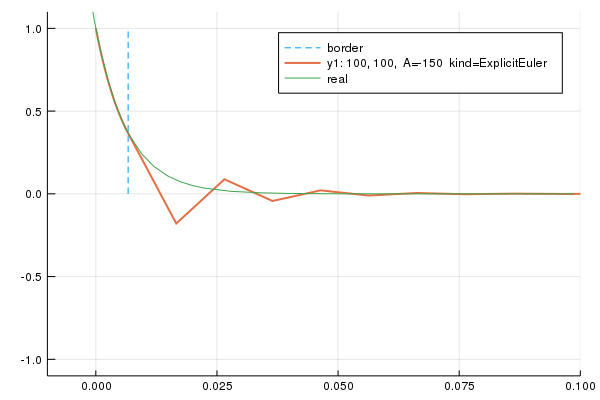
\includegraphics[width=0.5\pagewidth]{ode/stiff/exp-stiff-ExplicitEuler-1}

    \item  $A<0$, $\abs{Ah} \geqslant 2$. Тогда $1 + hA \leqslant -1$. Здесь колебания даже
      не затухают, а вообще растут. Что-то никак не связанное с экспонентой.

      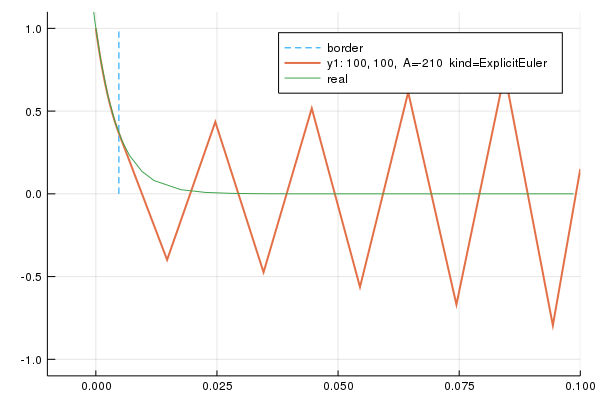
\includegraphics[width=0.5\pagewidth]{ode/stiff/exp-stiff-ExplicitEuler-2}
  \end{enumerate} 
\end{exmp}

\begin{exmp}\label{exmp:ode::stiff::linimpleuler}
  Снова рассмотрим $f(x, y) = A y$, $y(0)=1$ (всё одномерное). Его решение~"--- $y=e^{Ax}$.

  Попробуем решить неявным методом Эйлера
  \[
    y_{n+1} = y_n + hAy_{n+1} \so y_{n+1} = \frac{1}{1-Ah}\, y_n =
    \left(\frac{1}{1-Ah}\right)^{n+1} y_0
  \]
   
  И вот здесь никаких проблем c $A < 0$ нету, какое бы оно большое не было.
  Сравним его с явным методом Эйлера

  \noindent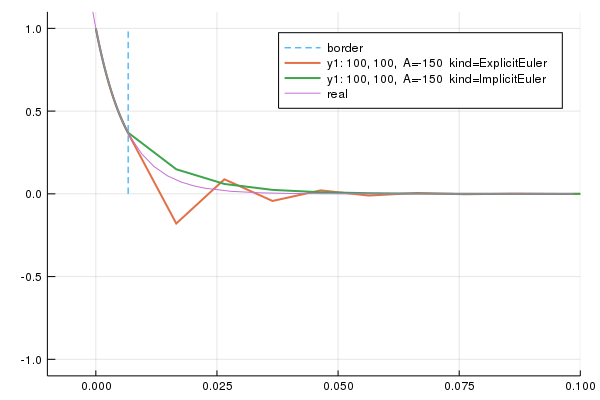
\includegraphics[width=0.5\textwidth]{ode/stiff/exp-stiff-Eulers-1}
  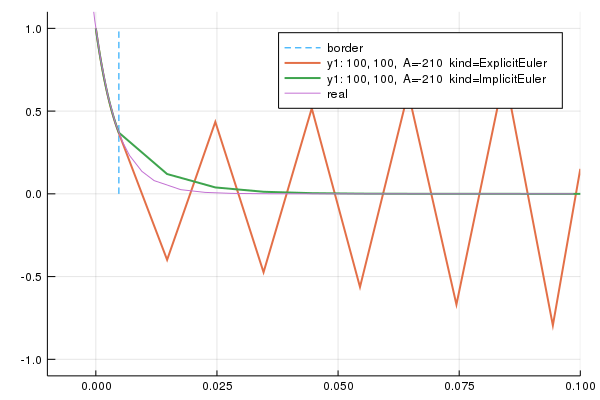
\includegraphics[width=0.5\textwidth]{ode/stiff/exp-stiff-Eulers-2}
\end{exmp}

\begin{defn}\label{defn:ode::stiff::R}
  Рассмотрим одношаговый метод для $y'=Ay$, $R(z) \that y_{n+1} = R(Ah) y_{n}$~"--- функция
  устойчивости \quest переходный множитель \quest \underdev
\end{defn}

\begin{defn}\label{defn:ode::stiff::astab}
  Одношаговый метод называется $A$-устойчивым, если для него $\abs{R(z)} \leqslant 1$ в 
  левой полуплоскости.
\end{defn}

\begin{defn}\label{defn:ode::stiff::astabarea}
  $\{ z \mid \abs{R(z) \leqslant 1} \leqslant 1\}$ называется областью $A$-устойчивости метода. 
\end{defn}

\begin{exmp}\label{exmp:ode::stiff::expeulerstabarea}
  Явный метод Эйлера устойчив в круге $\abs{z+1} < 1$: для него $R(z) = 1 + z$.
\end{exmp}

\paragraph{Неявные методы Рунге-Кутты}
\begin{defn}\label{defn:ode::stiff::astab}
  Одношаговый метод называется $L$-устойчивым, если он $A$-устойчив и 
  \hbox{$\lim\limits_{z\to\infty} R(z) = 0$}.
\end{defn}
например, тот же неявный метод Эйлера.

\label{par:ode::stiff}


\end{document}


% vim:wrapmargin=3
